\documentclass[11pt]{article}
\usepackage[T1]{fontenc}
\usepackage[utf8]{inputenc}

\PassOptionsToPackage{hyphens}{url}
\usepackage[
colorlinks=true,linkcolor=blue,urlcolor=blue,citecolor=blue,bookmarks=true,
bookmarksopenlevel=2]{hyperref}
\usepackage{cleveref}
\usepackage{graphicx}
\usepackage{geometry}
\geometry{%total={210mm,297mm},
left=25mm,right=25mm,%
bindingoffset=0mm, top=20mm,bottom=20mm}

\setlength\parindent{0pt}
\setlength{\parskip}{1mm}

\sloppy

\title{Overview of Multi-Agent Path Finding (MAPF)}
\author{Wolfgang Hönig\footnote{Now at California Institute of Technology}, Jiaoyang Li, Sven Koenig --- University of Southern California}
\date{Model AI 2020 Assignments: A Project on Multi-Agent Path Finding (MAPF)}

\begin{document}
\maketitle

\section{Introduction \label{intro}}

\begin{figure}[ht]
\centering
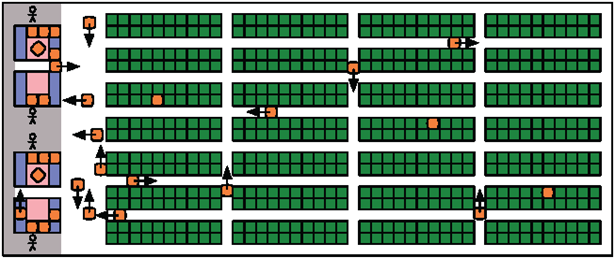
\includegraphics[width=0.5\textwidth]{images/amazon-warehouse.png}
\caption{A small Amazon order-fulfillment center~\protect\cite{kiva}.}\label{fig:kiva}
\end{figure}

\emph{Multi-agent path finding (MAPF)} is important for many applications, including automated warehousing. For example, Amazon order-fulfillment centers (Figure~\ref{fig:kiva}) have inventory stations around the perimeter of the warehouse (shown only on the left side in the figure) and storage locations in its center. Each storage location can store one inventory pod. Each inventory pod holds one or more kinds of goods. A large number of warehouse robots operate autonomously in the warehouse. Each warehouse robot is able to pick up, carry, and put down one inventory pod at a time. The warehouse robots move inventory pods from their storage locations to the inventory stations where the needed goods are removed from the inventory pods (to be boxed and eventually shipped to customers) and then back to the same or different empty storage locations to return the inventory pods \cite{kiva}. Amazon puts stickers onto the floors of their order-fulfillment centers to delineate a grid and allow for robust robot navigation. However, path planning for the robots is tricky since most warehouse space is used for storage locations, resulting in narrow corridors where robots that carry inventory pods cannot pass each other. Just-in-time manufacturing is an extension of automated warehousing for which no commercial installations exist so far. For just-in-time manufacturing, there are manufacturing machines around the perimeter of the warehouse rather than inventory stations. Robots go back and forth between the warehouse and the manufacturing machines, transporting raw material in one direction and manufactured products in the other direction. Just-in-time manufacturing increases the importance of delivering all needed raw material almost simultaneously to the manufacturing machines.

The MAPF problem is a simplified version of these and many other multi-robot or multi-agent path-planning problems and can be described as follows: On math paper, some cells are blocked. The blocked cells and the current cells of $n$ agents are known. A different unblocked cell is assigned to each agent as its goal cell. The problem is to move the agents from their current cells to their respective goal cells in discrete time steps and let them wait there. The optimization objective is to minimize the sum of the travel times of the agents until they reach their goal cells (and can stay there forever). At each time step, each agent can \emph{wait} at its current cell or \emph{move} from its current cell to an unblocked neighboring cell in one of the four main compass directions. A \emph{path} for an agent is a sequence of move and wait actions that lead the agent from its start cell to its goal cell or, equivalently, the sequence of its cells at each time step (starting with time step 0) when it executes these actions. The length of the path is the travel time of the agent until it reaches its goal cell (and stays there forever afterward). A \emph{solution} is a set of $n$ paths, one for each agent. Its cost is the sum of the lengths of all paths. Agents are not allowed to collide with the environment or each other. Two agents collide if and only if they are both in the same cell at the same time step (called a \emph{vertex collision} or, synonymously a vertex conflict) or both move to the current cell of the other agent at the same time step (called an \emph{edge collision} or, synonymously, an edge conflict).  (An agent is allowed to move from its current cell $x$ to the current cell $y$ of another agent at the same time step when the other agent moves from cell $y$ to a cell different from cells $x$ and $y$.) Finding optimal collision-free solutions is NP-hard \cite{Yu13}.

\section{MAPF Example}

\begin{figure}[ht]
\centering
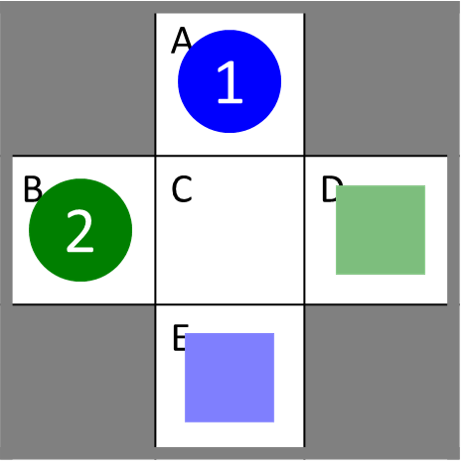
\includegraphics[width=0.2\textwidth]{images/example.png}
\caption{Our example MAPF instance. Circles represent start cells. Squares represent goal cells. \label{example}}
\end{figure}

Figure~\ref{example} shows an example MAPF instance with two agents, where agent 1 has to navigate from its current cell A to its goal cell E and agent 2 has to navigate from its current cell B to its goal cell D. One optimal collision-free solution (of cost 5) consists of path [A, C, E] (of length 2) for agent 1 and path [B, B, C, D] (of length 3) for agent 2. The other optimal collision-free solution (also of cost 5) consists of path [A, A, C, E] (of length 3) for agent 1 and path [B, C, D] (of length 2) for agent 2.

\section{Planning in Joint Location Space}

\begin{figure}[ht]
\centering
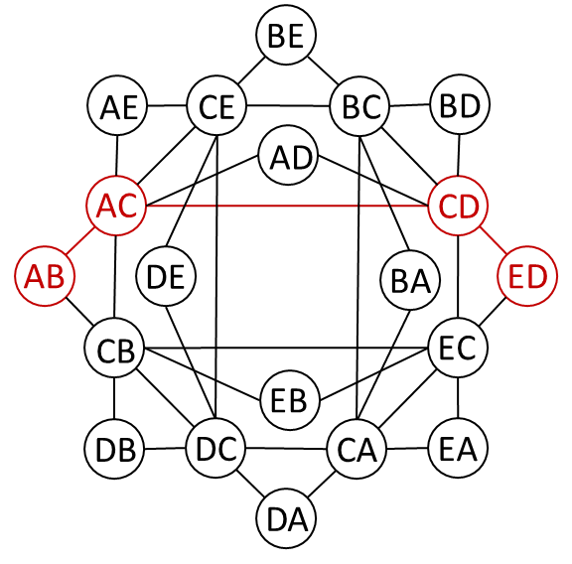
\includegraphics[width=0.35\textwidth]{images/joint-space.png}
\caption{The joint location space for our example MAPF instance, which contains 20 vertices and 36 edges. The two letters in each circular vertex represent the cells of agents 1 and 2. The red circles and lines represent an optimal solution, namely path [A, A, C, E] (of length 3) for agent 1 and path [B, C, D] (of length 2) for agent 2. }\label{fig:joint-space}
\end{figure}

In principle, one can find an optimal collision-free solution for a MAPF instance by planning for all agents simultaneously in joint location space by finding a shortest path on a graph whose vertices correspond to tuples of cells, namely one for each agent. Figure~\ref{fig:joint-space} shows this graph for our example MAPF instance. However, the number of vertices of the graph grows exponentially with the number of agents, which makes this search algorithm too slow in practice. Therefore, one needs to develop search algorithms that exploit the problem structure better to gain efficiency. We now discuss two such search algorithms, namely prioritized planning and conflict-based search.

\section{Prioritized Planning}

\emph{Prioritized planning} \cite{Erdm87} orders the agents completely by assigning each agent a different priority. It then plans paths for the agents, one after the other, in order of decreasing priority. It finds a path for each agent that does not collide with the environment or the (already planned) paths of all higher-priority agents (which can be done fast). Prioritized planning is fast but suboptimal (meaning that it does not always find an optimal collision-free solution) and even incomplete (meaning that it does not always find a collision-free solution even if one exists). If it finds a solution, then the solution is collision-free but the cost of the solution depends heavily on the priorities of the agents. More information on prioritized planning can be found in \cite{Ma19}.

Consider our example MAPF instance, and assume that agent 1 is assigned a higher priority than agent 2. Then, prioritized planning first finds the shortest path [A, C, E] (of length 2) for agent 1 and afterward the shortest path [B, B, C, D] (of length 3) for agent 2 that does not collide with the path of agent 1 (resulting in a collision-free solution of cost 5).


\begin{figure}[ht]
\centering
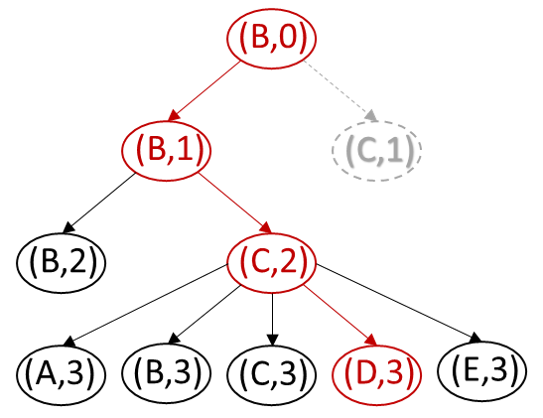
\includegraphics[width=0.3\textwidth]{images/space-time-A.png}
\caption{The search tree of space-time A* for agent 2 for our example MAPF instance if agent 1 has higher priority than agent 2 and the path of agent 1 is [A, C, E]. The pair in each oval node represents a cell and time step. The f-value of a node is the sum of its g-value (equal to the time step) and its h-value (equal to the distance of its cell to the goal cell D in the environment). Node (C,1) is pruned because agent 1 occupies cell C at time step 1 and agent 2 has to prevent a vertex collision with agent 1. The red nodes and edges represent an optimal solution for agent 2, namely path [B, B, C, D].}\label{fig:space-time-A}
\end{figure}

Prioritized planning uses \emph{space-time A*}~\cite{Silver05} to plan paths for each agent. Space-time A* is a modified A* algorithm that searches in the cell-time space, where the vertices are pairs $(x,t)$ of cells $x$ and time steps $t$. Vertex $(x,t)$ has a directed edge to vertex $(x, t+1)$ if and only if the agent can wait at cell $x$ at time step $t$. Vertex $(x,t)$ has a directed edge to vertex $(y, t+1)$ if and only if the agent can move from cell $x$ to cell $y \neq x$ from time step $t$ to time step $t+1$. \Cref{fig:space-time-A} shows the search tree of space-time A* for agent 2 for our example MAPF instance.

\section{Conflict-Based Search \label{cbs}}

\emph{Conflict-Based Search} (CBS)~\cite{Feln12,Feln15} first plans shortest paths for all agents independently (which can be done fast). These paths do not collide with the environment but are allowed to collide with the paths of the other agents. If this results in a collision-free solution, then it has found an optimal collision-free solution. Otherwise, it chooses a collision between two agents (for example, agents $a$ and $b$ are both in cell $x$ at time step $t$) and considers recursively two cases, namely one with the (negative) constraint that prohibits agent $a$ from being in cell $x$ at time step $t$ and one with the (negative) constraint that prohibits agent $b$ from being in cell $x$ at time step $t$. The hope is that CBS finds a collision-free solution before it has imposed all possible constraints. CBS is slower than prioritized planning but complete and optimal. CBS is a two-level search algorithm. We now describe its operation in detail.

The high level of CBS searches the binary {\em constraint tree}. Each node $N$ of the constraint tree contains: {\bf (1)} a set of constraints imposed on the agents, where a constraint imposed on agent $a$ is either a (negative) \emph{vertex constraint} $\langle a,x,t \rangle$, meaning that agent $a$ is prohibited from being in cell $x$ at time step $t$, or an (negative) \emph{edge constraint} $\langle a,x,y,t \rangle$, meaning that agent $a$ is prohibited from moving from cell $x$ to cell $y$ at time step $t$; {\bf (2)} a solution that satisfies all constraints but is not necessarily collision-free; and {\bf (3)} the cost of the solution. The root node of the constraint tree contains an empty set of constraints and a solution that consists of $n$ shortest paths. The high level performs a best-first search on the constraint tree, always choosing a fringe node of the constraint tree with the smallest cost to expand next. It breaks ties in favor of a node whose paths have fewer collisions with each other.

Once CBS has chosen node $N$ for expansion, it checks whether the solution of node $N$ is collision-free. If so, then node $N$ is a goal node and CBS returns its solution. Otherwise, CBS chooses one of the collisions and resolves it by {\em splitting} node $N$. Assume that CBS chooses to resolve a vertex collision where agents $a$ and $b$ are both in cell $x$ at time step $t$. In any collision-free solution, at most one of the agents can be in cell $x$ at time step $t$. Therefore, at least one of the constraints $\langle a,x,t \rangle$ (that prohibits agent $a$ from being in cell $x$ at time step $t$) or $\langle b,x,t \rangle$ (that prohibits agent $b$ from being in cell $x$ at time step $t$) must be satisfied. Consequently, CBS splits node $N$ by generating two child nodes of node $N$, each with a set of constraints that adds one of these two constraints to the constraint set of node $N$. Now assume that CBS chooses to resolve an edge collision where agent $a$ moves from cell $x$ to cell $y$ and agent $b$ moves from cell $y$ to cell $x$ at time step $t$. Then, the two additional constraints are the two edge constraints $\langle a,x,y,t \rangle$ (that prohibits agent $a$ from moving from cell $x$ to cell $y$ at time step $t$) and $\langle b,y,x,t \rangle$ (that prohibits agent $b$ from moving from cell $y$ to cell $x$ at time step $t$). 

For each child node, the low level of CBS finds a new shortest path for the agent with the newly imposed constraint, which can be done fast with space-time A* (as explained earlier and also in \cite{Feln15}). A vertex constraint, for example, just prunes a particular node in the search tree. This path does not collide with the environment and has to obey all constraints imposed on the agent in the child node but is allowed to collide with the paths of the other agents. 

\begin{figure}[ht]
\centering
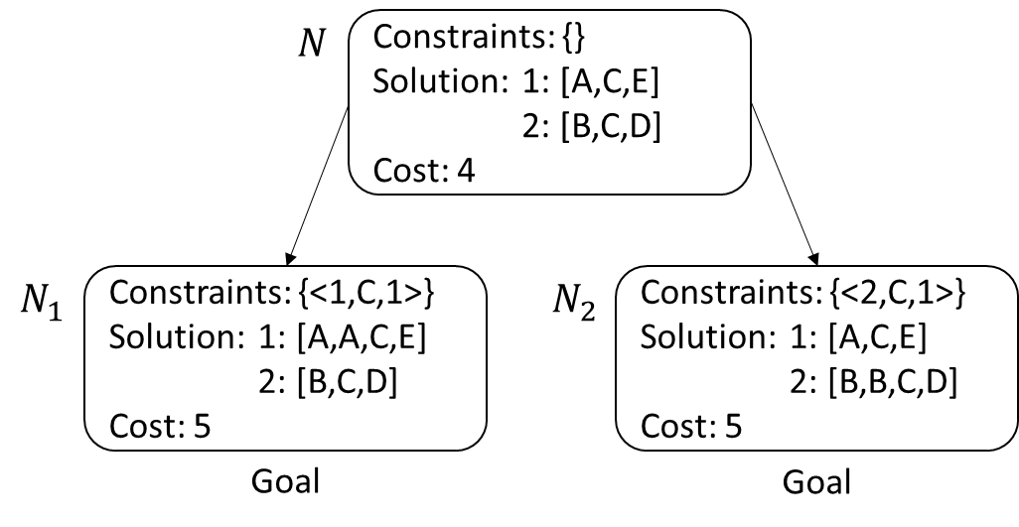
\includegraphics[width=0.5\textwidth]{images/CT.png}
\caption{Constraint tree for our example MAPF instance. \label{ct}}
\end{figure}

Consider our example MAPF instance. Figure~\ref{ct} shows the corresponding constraint tree. Its root node N contains the empty set of constraints, and the low level of CBS finds the shortest path [A, C, E] (of length 2) for agent 1 and the shortest path [B, C, D] (of length 2) for agent 2. Thus, the cost of node N is $2+2=4$. The solution of node N has a vertex collision where agents 1 and 2 are both in cell C at time step 1. Consequently, CBS splits node N. The new left child node N$_1$ of node N adds the constraint $\langle 1, C, 1 \rangle$. The low level of CBS finds the new shortest path [A, A, C, E] of length 3 (that includes a wait action) for agent 1 in node N$_1$, while the shortest path of agent 2 is identical to the one of node N since no new constraints have been imposed on agent 2. Thus, the cost of node N$_1$ is $3+2=5$. Similarly, the new right child node N$_2$ of node N adds the constraint $\langle 2, C, 1 \rangle$. The low level of CBS finds the new shortest path [B, B, C, D] of length 3 (that includes a wait action) for agent 2 in node N$_2$, while the shortest path of agent 1 is identical to the one of node N since no new constraints have been imposed on agent 1. Thus, the cost of node N$_2$ is $2+3=5$. The best-first search on the high level of CBS now chooses a fringe node of the constraint tree with the smallest cost to expand next. Assume that it breaks the tie between nodes N$_1$ and N$_2$ in favor of node N$_1$. Since the solution of node $N_1$ is collision-free, it is a goal node and CBS returns its collision-free solution (of cost 5) that consists of path [A, A, C, E] (of length 3) for agent 1 and path [B, C, D] (of length 2) for agent 2.

\section{Additional Information}

Additional information on the MAPF problem and solution approaches can be found at \url{http://mapf.info}, a website that contains tutorials, publications, data sets, and additional software for MAPF.

\section{Acknowledgments}

We thank NSF and Amazon for funding our work on this project material. 
We took the text of \cref{intro} almost verbatim from our previous research publication \cite{Ma17b} and the text of \cref{cbs} almost verbatim from our previous research publication \cite{Feln18}. We tested parts of this project at the Third Summer School on Cognitive Robotics, which was held from July 17 to July 21, 2019 at the University of Southern California, and the undergraduate "Introduction to Artificial Intelligence" class (CS360), which was held in Fall 2019 at the University of Southern California.

\bibliography{references}
\bibliographystyle{plain}

\end{document}

